%% ------------------------------------------------------------------------- %%
\chapter{Conceitos}
\label{cap:conceitos}


\section{Aprendizado Automático}

O campo de Aprendizado Automático (Machine Learning - ML) é um ramo da Ciência
da Computação que utiliza métodos estatísticos para criar sistemas que possam
aprender (i.e. melhorar sua acurácia) através de dados. Um problema de ML possui
as seguintes partes \citep{dlbook}: \\

\begin{itemize}

  
\item A tarefa $T$, no caso dos dados da Intercement, um problema de regressão.
  Onde desejamos estimar valores numéricos a partir de uma matriz de dados $X$ e
  suas anotações numéricas $Y$.  
  
\item Uma métrica de performance $P$, que define a distância entre as predições
  do modelo e os dados de treinamento. A teoria por trás desses métricas será explicada na seção~\ref{sec:metricas}.

\item A experiência $E$, que define qual tipo de informação o modelo poderá usar
  durante o treinamento. Explicaremos esse conceito na seção~\ref{sec:exp} 
  
\end{itemize}

\subsection{Aprendizado}
\label{sec:exp}
Algoritmos de ML podem ser divididos nas categorias de aprendizado supervisionado, não supervisionado e aprendizado por reforço \citep{dlbook}. Técnicas dos dois primeiros tipos serão usadas para os dados da Intercement.


\subsubsection{Aprendizado Supervisionado}

Aprendizado Supervisionado consiste, do ponto de vista estatístico, em aprender uma distribuição
de probabilidade do tipo $p(y | x)$. Nos são fornecidos diversos vetores de
entrada $x$ associados a uma anotação $y$ e gostariamos de modelar essa relação
entre dados e anotações para que possamos anotar novos dados inéditos para os
modelos. Ou seja, para diversos exemplos de vetores
$x$ são fornecidas anotações $y$, e desejamos então criar predições de anotações
$y'$ para novas entradas $x'$.


\subsubsection{Aprendizado Não Supervisionado}

Para o caso de Aprendizado Não Supervisionado, mantendo a estrutura do exemplo
anterior, desejaríamos então modelar uma distribuição do tipo $p(x)$, onde temos
também diversos exemplos de vetores aleatórios $x$ e estamos estudando alguma propriedade importante dessa distribuição.



\subsection{Métrica de Performance}
\label{sec:metricas}
\subsubsection{Estatística Frequentista e Estatística Bayesiana}
 
Como nesse trabalho serão usados métodos de inferência Bayesiana aplicados a ML,
cabe então uma breve elaboração das diferenças entre as duas principais
vertentes da estatística. O seguinte desenvolvimento é retirado de \cite{dlbook}:\\

Digamos que exista um evento aleatório que tenha um resultado com probabilidade
$p$ de acontecer. A visão frequentista de probabilidades diz que, se pudéssemos repetir infinitas vezes esse evento, a proporção de vezes que esse resultado irá acontecer se aproximará arbitrariamente de $p$. E então entenderíamos a probabilidade $p$ meramente como uma proporção de resultados positivos em uma certa amostra de experimentos. Mas e se o evento não pudesse ser repetido? Quando físicos criam modelos para explicar o nascimento do universo, é impossível pensar em repetir o Big Bang infinitas vezes para que se possam estimar probabilidades de certos eventos cosmológicos acontecerem. Nesse segundo caso, resultados são derivados de \textbf{graus de certeza}, onde a chance de um evento acontecer é estimada pela aplicação de conhecimentos prévios em vista de algo que foi observado posteriormente. A primeira maneira de se entender estatística é chamada de Frequentista e a segunda de Bayesiana. \\

E no campo de ML, as duas maneiras de se gerar predições são estimadores frequentistas e inferência Bayesiana \citep{dlbook}.

\subsubsection{Estimação por Log-verossimilhança}
 
Um exemplo de estimação frequentista que será usada nesse trabalho é a de
log-verossimilhança \citep{dlbook}. O desenvolvimento a seguir será feito para o
caso de distribuições de probabilidade que modelam problemas de aprendizado
\textbf{supervisionado}, e.g. $p(y|x)$. 
Essa estimação segue o princípio de maximizar a verossimilhança i.e. a probabilidade de
termos observado nossos dados \textit{com as anotações corretas}, parametrizada pelos parâmetros $\theta$: $p(y|x ; \theta)$.
Ou seja, dada uma matriz de dados $X$, suas anotações $Y$ e um conjunto de parâmetros $\theta$, o estimador de máxima verossimilhança de $\theta$ é dado por: \\

\[ \hat{\theta} = \argmax_{\theta} p_{modelo}(Y | X;\theta) \] 

Onde $p_{modelo}$ busca aproximar a real distribuição geradora dos dados $p$. Assumindo dados i.i.d e trocando a multiplicação por soma de logaritmos obtém-se: \\

\[ \hat{\theta} = \argmax_{\theta} \sum_{i=1}^{m} \log p_{modelo}(y^{(i)}| x^{(i)};\theta) \]

Maximizar a equação anterior é equivalente a minimizar a \textit{entropia-cruzada} entre
nossas anotações reais $y$ e as predições feitas pelo modelo $\hat{y}$
\citep{dlbook}. \\

Continuando com o caso de de aprendizado supervisionado, a \textit{entropia de uma variável aleatória} $y | x$ cuja função densidade
de probabilidade seja $p(y | x)$ pode ser calculada por \citep{shannon2001mathematical}: \\

\[ H(y | x)  = - \sum^m_{i=1} p(y_i | x_i)*\log p(y_i | x_i) \]

Ou ainda:

\[H(y | x) = - \mathop{\mathbb{E}}_p[\log p(y | x)] \]

Com o operador $\mathop{\mathbb{E}}_p[x]$ representando o valor esperado da
variável aleatória $x$ na distribuição $p$. \\

Sejam $p,p_{modelo}$ duas funções de distribuição de probabilidade. A \textit{entropia-cruzada} de $p_{modelo}$ em $p$ é definida pelo valor
esperado da entropia de $p_{modelo}$ na distribuição $p$ \citep{bayesml}: \\

\[H(p,p_{modelo}) =  \mathop{\mathbb{E}}_p[\log p_{modelo}(y | x)] \]

Se a distribuição $p_{modelo}$ for parametrizada pelo vetor $\theta$, a equação
acima toma a forma: \\


\[H(p,p_{modelo}) =  \mathop{\mathbb{E}}_p[\log p_{modelo}(y | x ; \theta)] \]

Minimizar essa equação é equivalente a maximizar a equação da
log-verossimilhança \citep{dlbook}. A sessão~\ref{sec:reglog} irá mostrar o caso
específico de estimação por log-verossimilhança para problemas de regressão.  

\subsubsection{Estimação por Log-verossimilhança para Regressão}
\label{sec:reglog}
Nos modelos usados nesse trabalho, a equação que irá ditar o \textbf{erro} a ser
minimizado pelos algoritmos é o MSE (explicado na sessão~\ref{sec:MSE}). 
É simples mostrar intuitivamente que minimizar o MSE entre os valores previstos
e os dados de treino pode ser considerado uma estimação por maximização de
verossimilhança \citep{dlbook}. É possível explicar uma regressão linear como
uma maximização de verossimilhança:
\\

Desejamos criar um modelo linear que explica a relação entre duas variáveis
$x$ e $y$ em um modelo da forma $y = \theta X + \epsilon$, onde $\epsilon
\sim \mathcal{N}(\epsilon;0,\,\sigma^2)$ e $\sigma$ é suposto conhecido.\\

Considera-se que esse modelo está produzindo uma distribuição condicional
$p(y|x)$ (assim como a maior parte dos problema de aprendizado supervisionado). \\ 

Define-se então, para esse modelo, $p(y|x) =
\mathcal{N}(y ; \hat{y}(x,\theta),\sigma^2)$, pois foi assumido que o ruído $\epsilon$
segue uma distribuição normal. Nota-se que a média da gaussiana é a previsão do
modelo. \\

A log-verossimilhança do modelo é dada por: \\

\[ LV =  \sum^m_{i=1}\log p(y_i | x_i ; \theta)\]


E como definimos a distribuição gerada pelo modelo como $
\mathcal{N}(y ; \hat{y}(x,\theta),\sigma^2)$, então usando a definição da
distribuição normal: \\

\[LV = -m \log \sigma - \frac{m}{2} \log (2 \pi) - \sum^m_{i=1}
  \frac{\abs{\hat{y_i}-y_i}^2}{2 \sigma^2} \]

Essa equação, ao ser otimizada, chega na mesma estimação de parâmetros $\theta$
que aplicar a equação do Erro Quadrático Médio \citep{dlbook}, explicada na seção~\ref{sec:MSE}.\\

\subsection{Função de Custo}

O \textit{aprendizado} de um modelo de ML consiste na busca por parâmetros que
minimizem alguma \textit{função de custo}. Normalmente algum algoritmo baseado
em gradientes aproxima os parâmetros maximizando a verossimilhança das predições
do modelo em relação aos dados observados. O que é equivalente a diminuir a
entropia cruzada entre a distribuição empírica dos dados e a distribuição
definida pelos parâmetros do modelo \citep{dlbook}. Nessa sessão iremos definir
a função de custo usada em todos os modelos de regressão usados, bem como a
métrica de acurácia, que testa a qualidade das predições dos modelos após o treinamento. \\

\subsubsection{R-quadrado}
Como teste da acurácia dos modelos foi usada a métrica R-quadrado \citep{cohen}. Sejam $\hat{y}$ e $y$ nossa previsão dada pelo modelo e o seu valor real, a acurácia do modelo é dada por:\\

\[R_2 = 1 - \frac{SS_{res}}{SS_{tot}}\]

\[SS_{tot} = \sum^n_{i=1} (y_i- \hat{y_i})^2\]

\[SS_{res} = \sum^n_{i=1} (y_i - \bar{y})^2\]

\[ \bar{y} = \frac{1}{n} \sum^n_{i=1} y\]

% \justify
Para essa métrica, o modelo pode ter um desempenho arbitrariamente ruim, com esse valor
podendo se tornar arbitrariamente negativo. Porém, seu valor máximo é 1,
indicando um modelo ideal.\\


\subsubsection{Erro Quadrático Médio}
\label{sec:MSE}
O erro quadrático médio (em inglês, MSE) é uma medida de diferença entre duas variáveis contínuas
$\hat{y}$ e y \citep{cohen}. Ele é dado por: \\

\[MSE = \sum^n_{i=1}\frac{(y_i - \hat{y_i})^2}{n}\]

Essa métrica é uma medida absoluta. E quanto maior esse valor pior o desempenho
do modelo. \\



%% ------------------------------------------------------------------------- %%

\section{Sequencialidade dos Dados}

Em um problema canônico de aprendizado supervisionado gostariamos de aprender
uma função $f$ tal que para um par inédito de dados $x^*,y^*$, a nossa função
dependa apenas de $x^*$ para gerar uma predição. Para os dados da Intercement pode ser que um valor i.e. índice de dureza dependa não só da última entrada, mas de diversas entradas anteriores. 

Ou seja, nossos dados podem ter sido gerados por uma distribuição de
probabilidade da forma $p(y | x_{t} ,x_{t -1},x_{t -2},x_{t-3} , \dots,
x_{t-T})$, onde uma saída $y$ é condicionada pelas últimas $T$ entradas. Para
resolver um problema de aprendizado dessa natureza, devemos usar \textbf{modelos
  sequenciais} \citep{dlbook}. 

Iremos então experimentar  modelos sequenciais e não-sequencias para testar a acurária de ambos no problema em questão.


\section{Modelos Usados} 

\subsection{Redes Neurais}


Redes neurais são aproximadores universais de funções \citep{nnuni}. Dado um problema
de classificação onde se deseja aprender uma função da forma $y = f^*(x)$, uma
Rede Neural define um mapeamento $y = f(x ; \theta)$, onde $\theta$ é o vetor de
parâmetros que serão aprendidos com o fim de minimizar a diferença entre a
distribuição empírica e essa distribuição gerada pelo modelo. Essa diferença pode
ser minimizada pelo método da verossimilhança, assim como elaborado na sessão~\ref{sec:reglog}.\\

O modelo neural é uma composição de funções que unem uma transformação linear e
a aplicação de uma função não-linear $\sigma$: \\

\[ f(x)=  \sigma(W*x + b) \]

Importante ressaltar que $W$ é uma matriz, assim como $x$ e $b$ são vetores. \\

A computação da saída de uma rede neural então pode ser escrita como:

\[   y = f_n \circ f_{n-1} \circ f_{n-2} \dots f_1(x)  \]

Para uma rede neural de $n$ \textbf{camadas}. Onde cada camada será uma função
$f_i$ cujos parâmetros são $W_i$ e $b_i$. Portanto, para a i-ésima camada da rede
sua saída será da forma: 

\[ f_i (x)=  a_i = \sigma(W_i*a_{i-1} + b_i) \]

Onde $a_{i-1}$ é a saída da camada anterior, também chamada de
\textbf{ativação}. A saída dessa camada é então a sua ativação $a_i$. \\ 

Vale notar que uma saída $y$ calculada por uma rede neural depende unicamente dos
seus parâmetros e da entrada $x$. Isso não será verdade para os modelos
\textbf{sequenciais} que também serão usados nesse trabalho, onde o estado
interno de computação desses modelos é usado como entrada para uma próxima
iteração \citep{dlbook}. \\

A seguir está reproduzida uma rede neural simples com uma camada oculta e dois neurônios de saída.


%\begin{figure}[H]
\centering

\scalebox{0.7}{
\begin{tikzpicture}[auto]

% operations =============================

% input layer
\node[op] (x5) {$x_5$};
\node[op, above=2.5pt of x5] (x4) {$Fe_2O_3$};
\node[op, above=2.5pt of x4] (x3) {$CaO$};
\node[op, above=2.5pt of x3] (x2) {$SiO_2$};
\node[op, above=2.5pt of x2] (x1) {$Al_2O_3$};
\node[op, below=2.5pt of x5] (x6) {$SO_3$};
\node[op, below=2.5pt of x6] (x7) {$P_2O_5$};
\node[op, below=2.5pt of x7] (x8) {$MgO$};
\node[op, below=2.5pt of x8] (x9) {$Na_2O$};
\node[op, below=2.5pt of x9] (x10) {$K_2O$};

% hidden layer
\node[op,  right=130pt of x5] (v2) {$v_2$};
\node[op, below=2.5pt of v2] (v3) {$v_3$};
\node[op, below=2.5pt of v3] (v4) {$v_4$};
\node[op, above=2.5pt of v2] (v1) {$v_1$};

\node[op,  right=40pt of v2] (h2) {$h_2$};
\node[op, below=2.5pt of h2] (h3) {$h_3$};
\node[op, below=2.5pt of h3] (h4) {$h_4$};
\node[op, above=2.5pt of h2] (h1) {$h_1$};


% output layer
\node[op,  right=60pt of h2] (z1) {$RC3$};
\node[op,  right=60pt of h3] (z2) {$RC7$};

%\node[op,  right=50pt of z1] (y1) {$\hat{y}_1$};
%\node[op,  right=50pt of z2] (y2) {$\hat{y}_2$};


% edges input layer to hidden
\path[tedge] (x1) -- (v1);
\path[tedge] (x1) -- (v2);
\path[tedge] (x1) -- (v3);
\path[tedge] (x1) -- (v4);

\path[tedge] (x2) -- (v1);
\path[tedge] (x2) -- (v2);
\path[tedge] (x2) -- (v3);
\path[tedge] (x2) -- (v4);

\path[tedge] (x3) -- (v1);
\path[tedge] (x3) -- (v2);
\path[tedge] (x3) -- (v3);
\path[tedge] (x3) -- (v4);

\path[tedge] (x4) -- (v1);
\path[tedge] (x4) -- (v2);
\path[tedge] (x4) -- (v3);
\path[tedge] (x4) -- (v4);

\path[tedge] (x5) -- (v1);
\path[tedge] (x5) -- (v2);
\path[tedge] (x5) -- (v3);
\path[tedge] (x5) -- (v4);

\path[tedge] (x6) -- (v1);
\path[tedge] (x6) -- (v2);
\path[tedge] (x6) -- (v3);
\path[tedge] (x6) -- (v4);

\path[tedge] (x7) -- (v1);
\path[tedge] (x7) -- (v2);
\path[tedge] (x7) -- (v3);
\path[tedge] (x7) -- (v4);

\path[tedge] (x8) -- (v1);
\path[tedge] (x8) -- (v2);
\path[tedge] (x8) -- (v3);
\path[tedge] (x8) -- (v4);

\path[tedge] (x9) -- (v1);
\path[tedge] (x9) -- (v2);
\path[tedge] (x9) -- (v3);
\path[tedge] (x9) -- (v4);

\path[tedge] (x10) -- (v1);
\path[tedge] (x10) -- (v2);
\path[tedge] (x10) -- (v3);
\path[tedge] (x10) -- (v4);

% edges hidden to hidden
\path[tedge] (v1) edge node[above=1pt] {{\Large$\sigma$}}  (h1) ;
\path[tedge] (v2) edge node[above=1pt] {{\Large$\sigma$}}  (h2) ;
\path[tedge] (v3) edge node[above=1pt] {{\Large$\sigma$}}  (h3) ;
\path[tedge] (v4) edge node[above=1pt] {{\Large$\sigma$}}  (h4) ;

% edges hidden to output
\path[tedge] (h1) -- (z1);
\path[tedge] (h1) -- (z2);

\path[tedge] (h2) -- (z1);
\path[tedge] (h2) -- (z2);

\path[tedge] (h3) -- (z1);
\path[tedge] (h3) -- (z2);

\path[tedge] (h4) -- (z1);
\path[tedge] (h4) -- (z2);

% edges output to output
%\path[tedge] (z1) edge node[above=1pt] {{\Large softmax}}  (y1) ;
%\path[tedge] (z2) edge node[above=1pt] {{\Large softmax}}  (y2) ;




\end{tikzpicture}
} % scalebox
\end{figure}


Na figura mostramos como seria uma rede que usa como parâmetros alguns dos dados de Farinha para modelar os índices RC3 e RC7 dos dados de expedição.

\bigskip


\subsection{Inferência Bayesiana em Machine Learning}
\label{sec:bayesinf}
O tratamento Bayesiano para modelos de ML é bastante diverso dos frequentistas \citep{dlbook}.
Em uma análise frequentista estima-se um valor de $\theta$ e então todas as
predições são feitas a partir desse valor. No caso Bayesiano se consideram todos
os possíveis valores de $\theta$ ao se fazer uma predição. É preciso especificar
um grau de certeza \textbf{a priori} $p(\theta)$ sobre os parâmetros, e então
consideramos que os dados \textbf{foram observados} e usamos a lei de Bayes para
calcular a \textbf{probabilidade} posterior $p(\theta | X,Y)$ usando para tal
$p(X,Y | \theta)$, a chamada verossimilhança \citep{bayesml}. 

\[    p(\theta | X,Y) = \frac{p(Y| X,\theta) p(\theta)}{p(Y)}   \]

Finalmente, para realizar uma inferência devemos integrar por toda a distribuição $p(\theta)$ marginalizando esse parâmetro. Se por exemplo queremos uma nova anotação $y^*$ para um novo dado $x^*$:

\[ p(y^* | x^* , X,Y) = \int  p(y^* | x^*,\theta) p(\theta | X,Y)  d\theta \]

Essa integral é geralmente intratável pela dificuldade de se calcular
analiticamente $p(\theta | X,Y)$ \citep{ubertime}, e portanto será usada uma
técnica que aproxima uma inferência Bayesiana numericamente em redes neurais, o Monte Carlo
Dropout \citep{dropbayes}. \\



O MC Dropout consiste no uso de \textbf{Dropout} em todas as camadas da rede
neural, i.e. descartar ativações aleatoriamente entre duas camadas da rede com
probabilidade $p$.\\

\begin{figure}
  



\begin{tikzpicture}

	\node[circle, draw, thick] (i1) {};
	\node[circle, draw, thick, above=2em of i1] (i2) {};
	\node[circle, draw, thick, above=2em of i2] (i3) {};
	\node[circle, draw, thick, below=2em of i1] (i4) {};
	\node[circle, draw, thick, below=2em of i4] (i5) {};
	
	\node[circle, draw, thick, right=4em of i1] (h1) {};
	\node[circle, draw, thick, right=4em of i2] (h2) {};
	\node[circle, draw, thick, right=4em of i3] (h3) {};
	\node[circle, draw, thick, right=4em of i4] (h4) {};
	\node[circle, draw, thick, right=4em of i5] (h5) {};
	
	\node[circle, draw, thick, right=4em of h1] (hh1) {};
	\node[circle, draw, thick, right=4em of h2] (hh2) {};
	\node[circle, draw, thick, right=4em of h3] (hh3) {};
	\node[circle, draw, thick, right=4em of h4] (hh4) {};
	\node[circle, draw, thick, right=4em of h5] (hh5) {};
	
	\node[circle, draw, thick, right=4em of hh2] (o1) {};
	\node[circle, draw, thick, right=4em of hh4] (o2) {};
	
	\draw[-stealth, thick] (i1) -- (h1);
	\draw[-stealth, thick] (i1) -- (h2);
	\draw[-stealth, thick] (i1) -- (h3);
	\draw[-stealth, thick] (i1) -- (h4);
	\draw[-stealth, thick] (i1) -- (h5);
	\draw[-stealth, thick] (i2) -- (h1);
	\draw[-stealth, thick] (i2) -- (h2);
	\draw[-stealth, thick] (i2) -- (h3);
	\draw[-stealth, thick] (i2) -- (h4);
	\draw[-stealth, thick] (i2) -- (h5);
	\draw[-stealth, thick] (i3) -- (h1);
	\draw[-stealth, thick] (i3) -- (h2);
	\draw[-stealth, thick] (i3) -- (h3);
	\draw[-stealth, thick] (i3) -- (h4);
	\draw[-stealth, thick] (i3) -- (h5);
	\draw[-stealth, thick] (i4) -- (h1);
	\draw[-stealth, thick] (i4) -- (h2);
	\draw[-stealth, thick] (i4) -- (h3);
	\draw[-stealth, thick] (i4) -- (h4);
	\draw[-stealth, thick] (i4) -- (h5);
	\draw[-stealth, thick] (i5) -- (h1);
	\draw[-stealth, thick] (i5) -- (h2);
	\draw[-stealth, thick] (i5) -- (h3);
	\draw[-stealth, thick] (i5) -- (h4);
	\draw[-stealth, thick] (i5) -- (h5);
	
	\draw[-stealth, thick] (h1) -- (hh1);
	\draw[-stealth, thick] (h1) -- (hh2);
	\draw[-stealth, thick] (h1) -- (hh3);
	\draw[-stealth, thick] (h1) -- (hh4);
	\draw[-stealth, thick] (h1) -- (hh5);
	\draw[-stealth, thick] (h2) -- (hh1);
	\draw[-stealth, thick] (h2) -- (hh2);
	\draw[-stealth, thick] (h2) -- (hh3);
	\draw[-stealth, thick] (h2) -- (hh4);
	\draw[-stealth, thick] (h2) -- (hh5);
	\draw[-stealth, thick] (h3) -- (hh1);
	\draw[-stealth, thick] (h3) -- (hh2);
	\draw[-stealth, thick] (h3) -- (hh3);
	\draw[-stealth, thick] (h3) -- (hh4);
	\draw[-stealth, thick] (h3) -- (hh5);
	\draw[-stealth, thick] (h4) -- (hh1);
	\draw[-stealth, thick] (h4) -- (hh2);
	\draw[-stealth, thick] (h4) -- (hh3);
	\draw[-stealth, thick] (h4) -- (hh4);
	\draw[-stealth, thick] (h4) -- (hh5);
	\draw[-stealth, thick] (h5) -- (hh1);
	\draw[-stealth, thick] (h5) -- (hh2);
	\draw[-stealth, thick] (h5) -- (hh3);
	\draw[-stealth, thick] (h5) -- (hh4);
	\draw[-stealth, thick] (h5) -- (hh5);
	
	
	\draw[-stealth, thick] (hh1) -- (o1);
	\draw[-stealth, thick] (hh1) -- (o2);
	\draw[-stealth, thick] (hh2) -- (o1);
	\draw[-stealth, thick] (hh2) -- (o2);
	\draw[-stealth, thick] (hh3) -- (o1);
	\draw[-stealth, thick] (hh3) -- (o2);
	\draw[-stealth, thick] (hh4) -- (o1);
	\draw[-stealth, thick] (hh4) -- (o2);
	\draw[-stealth, thick] (hh5) -- (o1);
	\draw[-stealth, thick] (hh5) -- (o2);
	
	\draw[-stealth, double, dashed, thick] (5.5,0) -- node[above] {dropout} (8.6, 0);
	
	
	%%% BOUNDARY %%%
	
	\node[circle, draw, thick, red, fill=red!10, right=15em of hh1] (i1) {};
	\node[circle, draw, thick, red, fill=red!10, above=2em of i1] (i2) {};
	\node[circle, draw, thick, above=2em of i2] (i3) {};
	\node[circle, draw, thick, below=2em of i1] (i4) {};
	\node[circle, draw, thick, below=2em of i4] (i5) {};
	
	\node[red] (icr) at (i1) {$\mathlarger{\mathlarger{\mathlarger{\mathlarger{\mathlarger{\bm{\times}}}}}}$};
	\node[red] (icr) at (i2) {$\mathlarger{\mathlarger{\mathlarger{\mathlarger{\mathlarger{\bm{\times}}}}}}$};
	
	\node[circle, draw, thick, red, fill=red!10, right=4em of i1] (h1) {};
	\node[circle, draw, thick, right=4em of i2] (h2) {};
	\node[circle, draw, thick, red, fill=red!10, right=4em of i3] (h3) {};
	\node[circle, draw, thick, red, fill=red!10, right=4em of i4] (h4) {};
	\node[circle, draw, thick, right=4em of i5] (h5) {};
	
	\node[red] (icr) at (h1) {$\mathlarger{\mathlarger{\mathlarger{\mathlarger{\mathlarger{\bm{\times}}}}}}$};
	\node[red] (icr) at (h3) {$\mathlarger{\mathlarger{\mathlarger{\mathlarger{\mathlarger{\bm{\times}}}}}}$};
	\node[red] (icr) at (h4) {$\mathlarger{\mathlarger{\mathlarger{\mathlarger{\mathlarger{\bm{\times}}}}}}$};
	
	\node[circle, draw, thick, right=4em of h1] (hh1) {};
	\node[circle, draw, thick, red, fill=red!10, right=4em of h2] (hh2) {};
	\node[circle, draw, thick, right=4em of h3] (hh3) {};
	\node[circle, draw, thick, red, fill=red!10, right=4em of h4] (hh4) {};
	\node[circle, draw, thick, right=4em of h5] (hh5) {};
	
	\node[red] (icr) at (hh2) {$\mathlarger{\mathlarger{\mathlarger{\mathlarger{\mathlarger{\bm{\times}}}}}}$};
	\node[red] (icr) at (hh4) {$\mathlarger{\mathlarger{\mathlarger{\mathlarger{\mathlarger{\bm{\times}}}}}}$};
	
	\node[circle, draw, thick, right=4em of hh2] (o1) {};
	\node[circle, draw, thick, right=4em of hh4] (o2) {};
	
	\draw[-stealth, thick] (i3) -- (h2);
	\draw[-stealth, thick] (i3) -- (h5);
	\draw[-stealth, thick] (i4) -- (h2);
	\draw[-stealth, thick] (i4) -- (h5);
	\draw[-stealth, thick] (i5) -- (h2);
	\draw[-stealth, thick] (i5) -- (h5);
	
	\draw[-stealth, thick] (h2) -- (hh1);
	\draw[-stealth, thick] (h2) -- (hh3);
	\draw[-stealth, thick] (h2) -- (hh5);
	\draw[-stealth, thick] (h5) -- (hh1);
	\draw[-stealth, thick] (h5) -- (hh3);
	\draw[-stealth, thick] (h5) -- (hh5);
	
	\draw[-stealth, thick] (hh1) -- (o1);
	\draw[-stealth, thick] (hh1) -- (o2);
	\draw[-stealth, thick] (hh3) -- (o1);
	\draw[-stealth, thick] (hh3) -- (o2);
	\draw[-stealth, thick] (hh5) -- (o1);
	\draw[-stealth, thick] (hh5) -- (o2);

\end{tikzpicture}


%%% Local Variables:
%%% mode: latex
%%% TeX-master: t
%%% End:

  \label{fig:dropout}
  \caption{Representacão do uso de Dropout em uma rede neural}
\end{figure}

Formalmente, para um vetor de ativações $a$ na saída de uma
camada da rede neural, amostramos um vetor de \textit{máscara} $r$ de uma
distribuição de Bernoulli cujo parâmetro é $p$, i.e. $r \sim Bernoulli(p)$.
Finalmente, o novo vetor de ativações é calculado por $r * a$. O efeito desse
processo é de zerar aleatoriamente entradas do vetor de ativação.
\\ 

\cite{dropbayes} demonstram que a aplicação do dropout em todas as camadas do
modelo equivale em aproximar numericamente uma distribuição $q(\theta)$ que
cumpriria o papel da distribuição intratável $p(\theta | X,Y)$ na inferência Bayesiana. \\

Para o cálculo da incerteza das predições do modelo se realizam então $B$ computações estocásticas de uma mesma
saída $y^*$, sejam elas $Y^* = \{y^*_{(1)},y^*_{(2)}, \dots , y^*_{(B)}\}$. A incerteza
  dessa medida é calculada então pela variância amostral de $Y^*$.



\subsection{Random Forest}

Random Forests são um método de \textbf{Ensemble Learning} para classificação ou regressão. \textbf{Ensemble Learning} é uma família de técnicas no qual diversos modelos "fracos" são usados em conjunto com algum sistema de votação para que a a acurária do sistema em conjunto se torne melhor que a de qualquer um dos modelos sozinho. Seguindo essa ideia, Random Forests são conjuntos de diveras árvores de decisão simples unidas por um meta-algoritmo de votação para que se produza uma predição muito mais eficaz.


\section{Modelos Sequenciais}
Com o sucesso de modelos sequenciais no campo do Deep Learning, iremos averiguar se é possível modelar sequencialmente os dados da produção de cimento usando dois desses modelos. 
\\

\subsection{Rede Neural Recorrente}
% 
\scalebox{1}{
\begin{tikzpicture}[auto]

% RNN state cell =============================
\node[state] (h) {$\vect{h}$};
\node[op, below=30pt of h] (x) {$\vect{x}$};
\node[op, above=30pt of h] (yhat) {$\hat{\vect{y}}$};



% edges
\path[tedge] (x) edge node[below right= -4pt] {$\vect{U}$}  (h) ;
\path[tedge] (h) edge [out=-400,in=-320,looseness=8, distance=125pt] node[above right] {$\vect{W}$} (h);
\path[tedge] (h) edge node[below right = -4pt] {$\vect{V}$} (yhat);


\end{tikzpicture}
} % scalebox


A família das Redes Neurais Recorrentes (RNN) é composta por modelos especializados
em processar dados sequenciais \citep{dlbook}, da forma $x^{(1)},x^{(2)} ,x^{(3)}\dots ,x^{(T)}$. Uma rede neural recorrente é definida por uma função com
\textbf{recorrência} ou \textbf{recursão}, de modo que no processamento de uma
sequência o estado da rede seja de certo modo propagado temporalmente. A equação
a seguir ilustra uma função com recorrência: \\

\[h^{(t)} = f(h^{(t-1)},x^{(t)};\theta)\]

Nessa equação notamos que na iteração $t$ o valor do vetor $h$ depende de
$h_{t-1}$.RNNs aprendem a usar esse vetores como
\say{resumos} das iterações passadas. Desse modo , o modelo ganha a capacidade
de usar informações passadas da sequência para o cálculo
de uma saída. Essa capacidade porém começa a ser dificultada quando o modelo
realiza muitas iterações temporais. Durante o aprendizado, sequências muito
extensas criam problemas numéricos para o cálculo dos gradientes, esses podendo
tomar valores muito pequenos ou muito grandes. Foram propostos outros modelos
que não possuam esse problema, como o modelo LSTM, explicado na sessão~\ref{sec:lstm}. 

%%%
\begin{figure}[H]
\centering
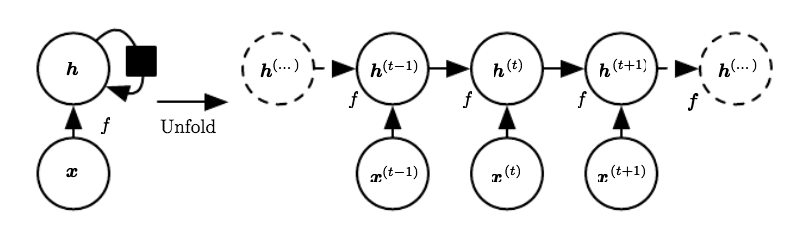
\includegraphics[width=0.9\columnwidth]{rnn.png}
\caption{Grafo de Computação de uma RNN genérica \citep{dlbook}}
\label{fig:rnngraph}
\end{figure}
%%%

Como podemos ver na Figura~\ref{fig:rnngraph}, a entrada $x$, ao lado do estado
interno $h$, são usados para calcular um novo estado. Nota-se que o vetor $h$,
bem como os parâmetros internos da RNN, são divididos entre iterações temporais.
\\

Essa classe de modelos normalmente é usada para modelagem de linguagem. Buscando
estimar uma distribuição de probabilidade $p(w_t | w_{t-1},w_{t-2},w_{t-3} \dots
) $ onde os $w_i$ são palavras subsequentes de um texto. Normalmente um modelo
dessa natureza busca resolver um problema de classifição, onde a próxima palavra
a ser prevista pelo modelo é uma entre todas as possibilidades de um certo
vocabulário. No caso do domínio em questão desejamamos resolver um problema de
regressão, onde nosso alvo é um valor numérico. Para treinar um desses modelos,
precisamos usar como entrada exemplos subsequentes de dados, onde cada exemplo
de entrada tem um exemplo pareado de saída. Basicamente redes neurais
recorrentes funcionam recebendo um exemplo de entrada, criando uma representação
interna com o mesmo e então gerando uma saída e comparando essa saída com o
exemplo de saída real, gerando um erro. Finalmente, esse erro é propagado para
alterar seus parâmetros (com o fim de achar um conjunto de parâmetros que gere
boas previsões). \\ 


Como já explicado anteriormente, nossos dados de entrada e saída não estão necessariamente pareados perfeitamente dia a dia. Portanto, foi necessário achar intervalos de tempo nos dados onde existe esse pareamento. Isso reduz drasticamente quais períodos representados nos dados realmente podem ser usados para treinar um desses modelos.


\subsubsection{LSTM}
\label{sec:lstm}

LSTMs \citep{lstm} são um tipo de RNN que por meio de sua arquitetura permitem que sequências
maiores sejam processadas sem que o fluxo dos gradientes propagados pela rede se torne
numericamente problemático (i.e. tendendo a 0 ou a infinito). A Figura~\ref{fig:lstm} ilustra o fluxo dos sinais em uma LSTM. \\
\begin{figure}
\centering
\caption{Diagrama da arquitetura de uma LSTM}


\begin{tikzpicture}[
    prod/.style={circle, draw, inner sep=0pt},
    ct/.style={circle, draw, inner sep=5pt, ultra thick, minimum width=10mm},
    ft/.style={circle, draw, minimum width=8mm, inner sep=1pt},
    filter/.style={circle, draw, minimum width=7mm, inner sep=1pt, path picture={\draw[thick, rounded corners] (path picture bounding box.center)--++(65:2mm)--++(0:1mm);
    \draw[thick, rounded corners] (path picture bounding box.center)--++(245:2mm)--++(180:1mm);}},
    mylabel/.style={font=\scriptsize\sffamily},
    >=LaTeX
    ]

\node[ct, label={[mylabel]Cell}] (ct) {$c_t$};
\node[filter, right=of ct] (int1) {};
\node[prod, right=of int1] (x1) {$\times$}; 
\node[right=of x1] (ht) {$h_t$};
\node[prod, left=of ct] (x2) {$\times$}; 
\node[filter, left=of x2] (int2) {};
\node[prod, below=5mm of ct] (x3) {$\times$}; 
\node[ft, below=5mm of x3, label={[mylabel]right:Forget Gate}] (ft) {$f_t$};
\node[ft, above=of x2, label={[mylabel]left:Input Gate}] (it) {$i_t$};
\node[ft, above=of x1, label={[mylabel]left:Output Gate}] (ot) {$o_t$};

\foreach \i/\j in {int2/x2, x2/ct, ct/int1, int1/x1,
            x1/ht, it/x2, ct/it, ct/ot, ot/x1, ft/x3}
    \draw[->] (\i)--(\j);

\draw[->] (ct) to[bend right=45] (ft);

\draw[->] (ct) to[bend right=30] (x3);
\draw[->] (x3) to[bend right=30] (ct);

\node[fit=(int2) (it) (ot) (ft), draw, inner sep=0pt] (fit) {};

\draw[<-] (fit.west|-int2) coordinate (aux)--++(180:7mm) node[left]{$x_t$};
\draw[<-] ([yshift=1mm]aux)--++(135:7mm);
\draw[<-] ([yshift=-1mm]aux)--++(-135:7mm);

\draw[<-] (fit.north-|it) coordinate (aux)--++(90:7mm) node[above]{$x_t$};
\draw[<-] ([xshift=1mm]aux)--++(45:7mm);
\draw[<-] ([xshift=-1mm]aux)--++(135:7mm);

\draw[<-] (fit.north-|ot) coordinate (aux)--++(90:7mm) node[above]{$x_t$};
\draw[<-] ([xshift=1mm]aux)--++(45:7mm);
\draw[<-] ([xshift=-1mm]aux)--++(135:7mm);

\draw[<-] (fit.south-|ft) coordinate (aux)--++(-90:7mm) node[below]{$x_t$};
\draw[<-] ([xshift=1mm]aux)--++(-45:7mm);
\draw[<-] ([xshift=-1mm]aux)--++(-135:7mm);
\end{tikzpicture}


%%% Local Variables:
%%% mode: latex
%%% TeX-master: '../quali'
%%% End:

\label{fig:lstm}
\end{figure}


Uma rede LSTM possui três \say{portas}. Cada porta possui duas matrizes $W,U$ e um
vetor $b$ de parâmetros. Uma iteração da LSTM começa com o cálculo dos sinais
$o_t,i_t,f_t$.\\

\[f_t = \sigma_g(W_fx_t + U_fh_{t-1} + b_f)\]
\[i_t = \sigma_g(W_ix_t + U_ih_{t-1} + b_i)\]
\[o_t = \sigma_g(W_ox_t + U_oh_{t-1} + b_o)\]

O diferencial de uma LSTM é a propagação do sinal $c_t$, a célula de memória.
Esse valor depende de $f_t$ e $i_t$, que influenciam em como o valor da
célula de memória será atualizado na presente iteração. A equação a seguir
mostra como o valor da célula de memória é calculado. Onde $\circ$ é o produto Hadamard, ou apenas multiplição entrada por entrada de
duas matrizes ou vetores. \\

\[c_t = f_t \circ c_{t-1} + i_t \circ \sigma_c(W_cx_t + U_ch_{t-1} + b_c)\]

Nota-se que $f_t$
define quanto do valor antigo da célula de memória deve participar no cálculo do
seu novo valor. 
Da mesma maneira $i_t$ define quanto da nova entrada deve ser usada no cálculo desse valor.
Em outras palavras, as portas $i_t$ e $f_t$ definem o quanto a LSTM deve,
respectivamente, \say{lembrar} e \say{esquecer}.


O novo estado da LSTM é então calculado por: \\
\[h_t = o_t \circ \sigma_h(c_t)\]




\subsubsection{Rede Encoder-Decoder}

Redes Encoder-Decoder são usadas para modelagem de sequência para
sequência, ou seja, para receber dados sequenciais como entrada e gerar
sequências como saída \citep{dlbook}. Esses modelos possuem duas partes, ambas compostas por
RNNs. \\

\begin{figure}[H]
\centering
\begin{tikzpicture}[font=\sffamily]
\node[fill=brown!90!black, text=white, font=\sffamily\small, inner sep=2pt] (a) {\begin{tabular}{@{}r@{}}-0.2\\-0.1\\0.1\\0.4\\-0.3\\1.1\end{tabular}};

\node[fit=(a.north) (a.south), inner sep=1pt, right=1mm of a, minimum width=2cm, label=center:Decoder] (dec) {};
\node[fit=(a.north) (a.south), inner sep=1pt, left=1mm of a, minimum width=2cm, label=center:Encoder] (enc) {};

\begin{scope}[on background layer]
\fill[cyan!30] (dec.north west)--([yshift=5mm]dec.north east)--([yshift=-5mm]dec.south east)--(dec.south west)--cycle;
\fill[cyan!30] (enc.north east)--([yshift=5mm]enc.north west)--([yshift=-5mm]enc.south west)--(enc.south east)--cycle;
\end{scope}

\node[right=1mm of dec, fill=blue, single arrow] (b) {\phantom{a}};
\node[align=left, right=1mm of b] {Sequência de\\ saída};

\node[left=1mm of enc, fill=blue, single arrow] (c) {\phantom{a}};
\node[align=left, left=1mm of c] {Sequência de\\ entrada};
\end{tikzpicture}
%%% Local Variables:
%%% mode: latex
%%% TeX-master: t
%%% End:

\caption{ Diagrama de Rede Encoder-Decoder.\\ Modificado de \cite{encdec}}

\end{figure}
  
O \textbf{encoder} é uma RNN que busca receber uma sequência de entrada de
tamanho arbitrário e gerar uma representação como saída, o seu estado interno,
representando em marrom no diagrama acima. O \textbf{Decoder} então recebe essa representação interna (também chamada
de \textit{codificação}) e usa-a para gerar saídas sequencialmente, podendo
então gerar essas sequências de duas formas: O Decoder pode usar as suas próprias saídas
como entrada para gerar a saída da próxima iteração temporal, ou então usar dados de treinamento como
entradas, essa última forma chamada de \textit{teacher forcing}. No diagrama
está indicado o acoplamento entre o decoder e o encoder. Essa codificação é apenas
um vetor (cuja dimensão é um \textit{hiper-parâmetro} de treinamento) que resume a
informação sequencial lida pelo encoder e a transmite para o decoder.
Hiper-parâmetros são parâmetros do problema de aprendizado que são definidos
pelo programador e não fazem parte dos valores aprendidos pelo algoritmo de
aprendizado. É comum que se realizem diversos experimentos com diferentes
valores de hiper-parâmetros e se escolha os que geraram melhores resultados. 
\\

Redes encoder-decoder são muito usadas para aprender \textit{representações} para os
dados. Isso quer dizer que as codificações da rede encoder-decoder são frutos de
transformações no espaço das entradas que buscam extrair a informação mais útil
para o objetivo do aprendizado. Podemos pensar nessas transformações como
mudanças de coordenadas nas quais estamos representando os dados. A
imagem~\ref{} ilustra essa ideia. Justamente o problema de aprender
representações estimulou desde 2006 uma redescoberta do DL \citep{dlbook}. Criar
operações que transformem os dados de entrada de modo a facilitar o aprendizado
pode levar anos se essa tarefa for colocada na mão de especialistas humanos
\citep{dlbook}, então é uma capacidade valiosa proporcionada por algoritmos de
DL como redes encoder-decoder. \\
\\



\subsubsection{Modelo Encoder-Decoder-Forecaster}

Iremos reproduzir nesse trabalho o modelo proposto em \cite{ubertime}. A
arquitetura consiste em uma rede \textbf{encoder-decoder} que aprende codificações da
série temporal (i.e. uma representacão que extraia informações úteis para o
problema) e então uma rede \textbf{forecaster} que usa essas codificações ao lado de
variáveis exógenas a série temporal para realizar predições.  


\begin{figure}[H]
\centering
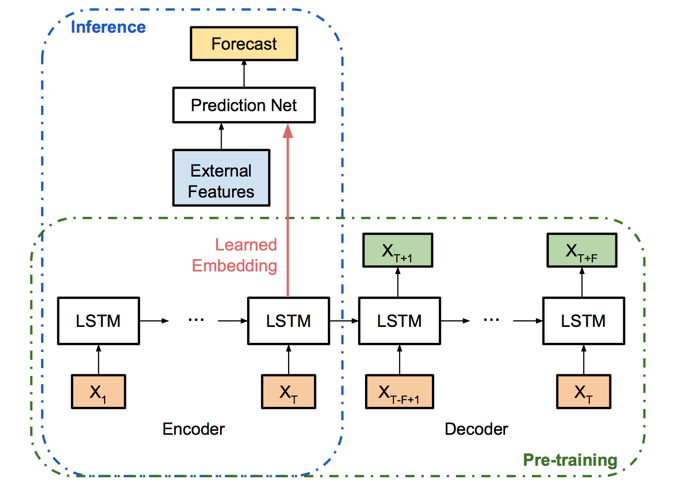
\includegraphics[width=0.9\columnwidth]{uber.png}
\caption{Arquitetura do modelo proposto por \cite{ubertime}}
\end{figure}


Durante o pré-treinamento a rede encoder-decoder consome sequências de $F$ dias
da série temporal. O encoder cria uma representação vetorial $h$ depois de
receber como entrada os primeiros $T$ ($T < F$) dias da sequência. Então, $h$ é usado como
inicialização do estado interno do decoder, e esse então consume mais $F - T$
entradas da sequência. Para o decoder, se em uma iteração sua entrada é $X_i$,
então sua saída será comparada com $X_{i+1}$, e esse erro é propagado após lidas
todas as entradas para que a representação $h$ proveniente do encoder possa se
tornar mais informativa.


Esse modelo também possui outra característica importante. Todas as camadas da
redes neurais que compõe o encoder, o decoder e o forecaster possuem
Dropout com probabilidade $p$. Ou seja, podemos usar a técnica do Monte
Carlo Dropout para estimar a variância de cada predição feita por esse modelo. A
rede então se torna um modelo bastante robusto para consumir séries temporais,
assim realizando predições e incertezas.\\


Essa capacidade do modelo o torna mais interessante do que meramente usar uma
rede LSTM para o problema de regressão. Agora iremos definir como a informação
de incerteza pode ser calculada usando esse modelo. \\

Na seção~\ref{sec:reglog} definimos um problema de regressão linear sob o ponto
de vista Bayesiano. De maneira similar, seja a distribuição gerada por esse
modelo $p(y | f^W(x))$. Onde $f^W$ denota a saída da
rede Forecaster após o treino. Como estamos lidando com regressão, assume-se: \\

 \[ y| W \sim \mathcal{N}( f^W(x),\,\sigma^2)\]

 Na seção~\ref{sec:bayesinf} explicamos como usamos inferência
 Bayesiana para marginalizar os parâmetros $W$ e calcular a distribuição $p(y^* | x^*)$
 A variância dessa distribuição quantifica a incerteza das predições
 \citep{dropbayes}, e pode ser decomposta usando a lei da variância total: \\


 %%%
 %%% nao omitir esse passo da derivação
 %%%
\[ Var(y^* | x^*) = Var(f^W(x^*)) + \sigma^2 \] 


Vemos que nossa incerteza é decomposta em dois termos. $Var(f^W(x^*))$ denota a
nossa ignorância em relação aos parâmetros do modelo, referida como
\textit{incerteza do modelo}. $\sigma^2$ seria então o \textit{ruído inerente} ao
processo gerador de dados.
 
A estimativa de $Var(f^W(x^*))$ se dá pela técnica do MC Dropout. A variância
será aproximada pela variância amostral de $B$ predições estocásticas calculadas
na rede com camadas de Dropout ativadas. Seja $\{\hat{y}^*_{(1)},\hat{y}^*_{(2)}, \dots
\hat{y}^*_{(B)}\}$ o vetor de predições amostrado dessa forma, e $\hat{y}^*$ sua
média amostral, temos: \\

\[   Var(f^W(x^*))  = \frac{1}{B}\sum^B_{B=1}(\hat{y}^*_{(B)} - \hat{y}^*)^2  \]


O ruído inerente das medidas é estimado usando os \textit{dados de validação},
i.e. aqueles não
usados durante o treinamento. Como
proposto por \citep{ubertime}, sejam $(X',Y')$ nossos dados de validação, com
$V$ entradas. Esses dados são independentes do nosso modelo
treinado $f^W(.)$, então podemos usa-los para estimar o ruído inerente do
modelo: \\

\[ \hat{\sigma}^2 = \frac{1}{V}\sum^V_{V=1}(y'_v - f^W(x'_v))^2 \]

Finalmente, sejam nossa incerteza do modelo $\eta_1^2$ e o ruído inerente
$\eta^2_2$, calcula-se a incerteza total do modelo por: \\

\[  \eta_{tot} = \sqrt{  \eta_1^2 + \eta_2^2 }  \]







%%% Local Variables:
%%% mode: latex
%%% TeX-master: "../quali"
%%% bibtex-file-path: "../bibliografia"
%%% End: